% ****** Start of file apssamp.tex ******
%
%   This file is part of the APS files in the REVTeX 4.1 distribution.
%   Version 4.1r of REVTeX, August 2010
%
%   Copyright (c) 2009, 2010 The American Physical Society.
%
%   See the REVTeX 4 README file for restrictions and more information.
%
% TeX'ing this file requires that you have AMS-LaTeX 2.0 installed
% as well as the rest of the prerequisites for REVTeX 4.1
%
% See the REVTeX 4 README file
% It also requires running BibTeX. The commands are as follows:
%
%  1)  latex apssamp.tex
%  2)  bibtex apssamp
%  3)  latex apssamp.tex
%  4)  latex apssamp.tex
%
\documentclass[%
 reprint,
%superscriptaddress,
%groupedaddress,
%unsortedaddress,
%runinaddress,
%frontmatterverbose,
%preprint,
%showpacs,preprintnumbers,
%nofootinbib,
%nobibnotes,
%bibnotes,
amsmath,amssymb,
%aps,
pra,
%prb,
%rmp,
%prstab,
%prstper,
%floatfix,
]{revtex4-1}

\usepackage{tabularx}
\usepackage{siunitx}
\usepackage{graphicx}% Include figure files
\usepackage{dcolumn}% Align table columns on decimal point
\usepackage{bm}% bold math
%\usepackage{hyperref}% add hypertext capabilities
%\usepackage[mathlines]{lineno}% Enable numbering of text and display math
%\linenumbers\relax % Commence numbering lines

%\usepackage[showframe,%Uncomment any one of the following lines to test
%%scale=0.7, marginratio={1:1, 2:3}, ignoreall,% default settings
%%text={7in,10in},centering,
%%margin=1.5in,
%%total={6.5in,8.75in}, top=1.2in, left=0.9in, includefoot,
%%height=10in,a5paper,hmargin={3cm,0.8in},
%]{geometry}

\begin{document}

\preprint{APS/123-QED}

\title{Raman characterization of CVD grown graphene \\and 2D material based heterostructures}% Force line breaks with \\

\author{Moritz Berger}
 \altaffiliation[]{RWTH Aachen University, Germany}%Lines break automatically or can be forced with \\
 \email{moritz.berger@rwth-aachen.de}
 \author{Gerald Kolter}
 \altaffiliation[]{RWTH Aachen University, Germany}%Lines break automatically or can be forced with \\
 \email{gerald.kolter@rwth-aachen.de}

%\date{May 1, 2019}
\date{\today}% It is always \today, today,
             %  but any date may be explicitly specified

%\begin{abstract}
%Pseudo-MOSFET structures have been investigated in recent years as they provide multiple applications. Additionally they can be used to determine relatively easily the charge carrier mobility $\mu _{eff}$ of different materials such as Si even in different configurations. In this paper a deeper look is given into important technologies used for fabricating Pseudo-MOSFETs, namely Optical Lithography and Reactive Ion Etching. Afterwards a set of devices is analyzed to characterize the output and transfer of the device, which give an indication of the quality of the device.
%\end{abstract}

\maketitle

\section{Introduction}
Novoselov et al. were the first to intentionally isolate a mono-layer of carbon atoms from a graphit block, called graphene.\citep{Novoselov2004} Since then it attracted an overwhelming interest in fundamental and applied research in a variety of fields, such as solid state physics, electronics, mechanics, and optics.\citep{NeumannStampfer} \\
Confocal Raman Spectroscopy provides the ability to obtain important material characteristics locally and noninvasively.\citep{NeumannStampfer} \\
Figure \ref{fig:Exfoliation_Spectra} shows Raman spectra analyzed later. One can mainly see three peaks. The high peak at about \SI{1600}{\per cm} is called the "G" peak, the lower peak at about \SI{2700}{\per cm} is called "2D" peak and the lowest peak at about \SI{2400}{\per cm} is called "D+D''" peak. The positions of the peak are denoted by $\omega _G$, $\omega _{2D}$ and $\omega _{D+D''}$ and the Full Width at Half Maximum (FWHM) are denoted by $\Gamma _G$, $\Gamma _{2D}$ and $\Gamma _{D+D''}$ respectively. \\
The G peak originates from the highest optical phonons at the $\Gamma$ point in the lattice. The 2D peak originates from the breathing mode of the TO branch around the K point in the lattice. The D+D'' originates from defects.\citep{NeumannStampfer}


\section{Exfoliation}
Exfoliation is the simplest technique to isolate graphene from a graphit block.

\subsection{Method}
In order to isolate a mono-layer of carbon atoms with exfoliation one uses a sticky tape and a graphit block. The first step is to place the graphit onto the sticky tape and pull it off again. After this one can see a film of graphit on the sticky tape. The second step is to press a sticky tape on the graphit film and pull it off again. This second step is repeated until one gets a mono-layer of carbon atoms.

\subsection{Results}

\begin{figure}
\centering
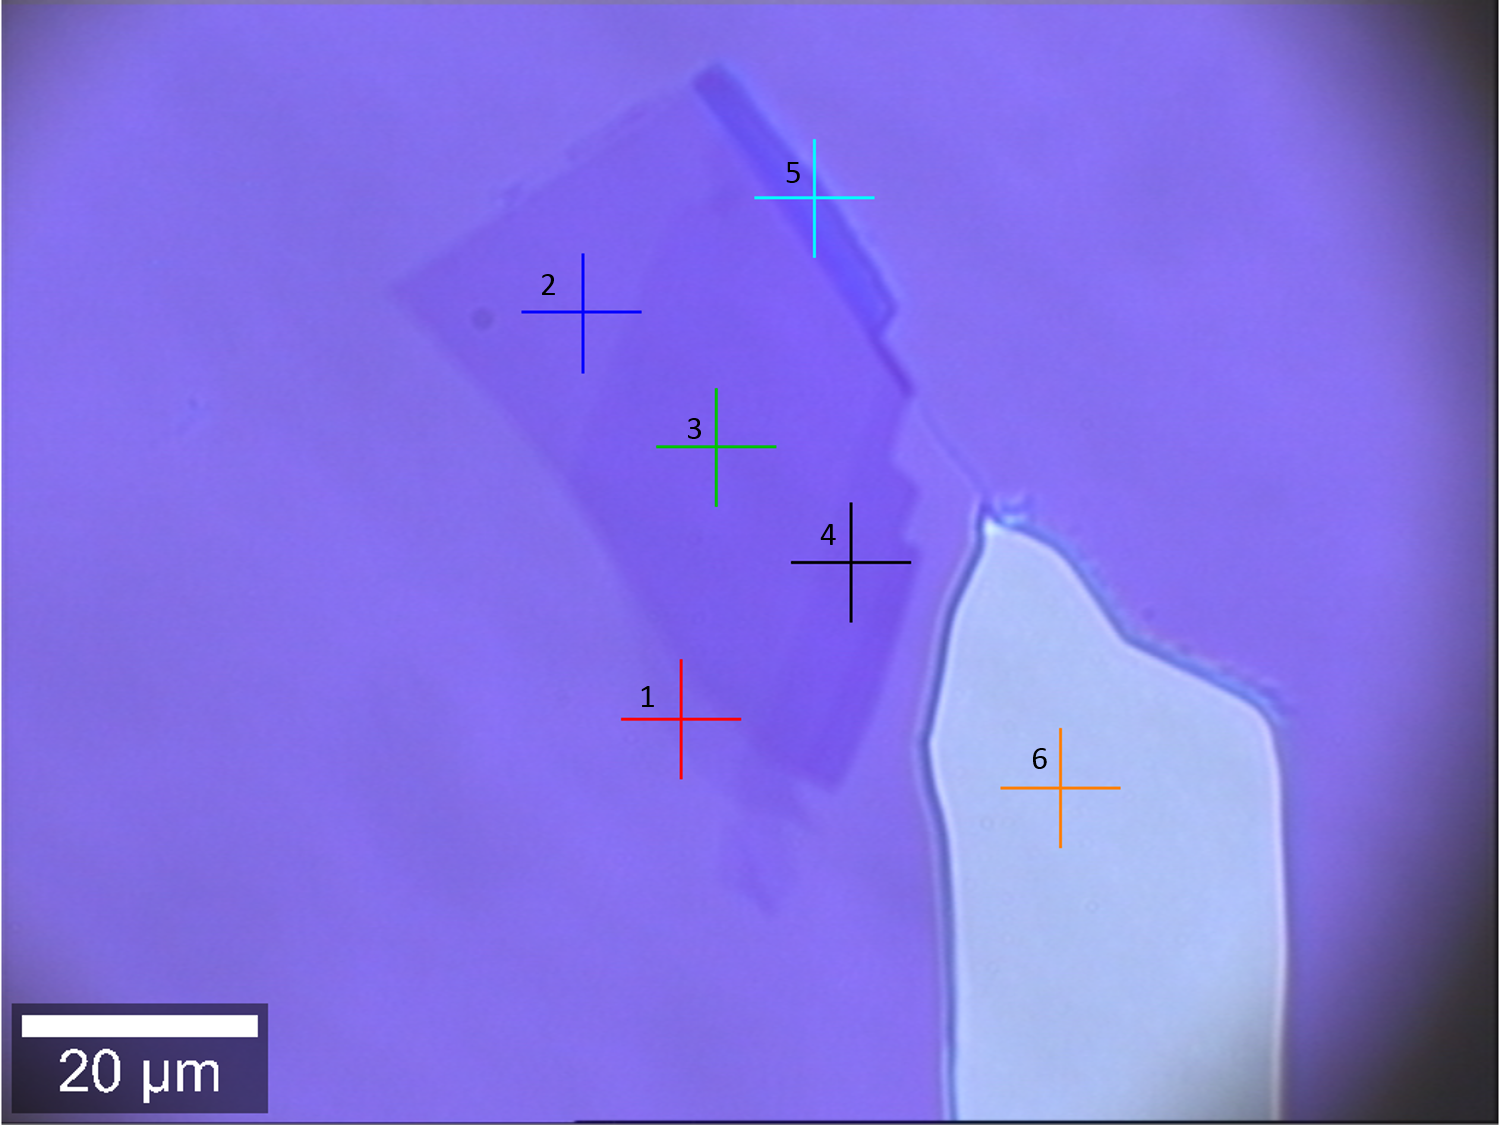
\includegraphics[scale=0.35]{Bilder/Exfoliation/mono_bi_tri_flake.PNG}
\caption{Image from one flake of graphene isolated by Exfoliation made with an optical microscope. The crosses mark the points where the Raman spectra are extracted.}
\label{fig:Exfoliation_Microscope}
\end{figure}

Figure \ref{fig:Exfoliation_Microscope} shows one of the flakes obtained by Exfoliation made with an optical microscope. This flake shows different numbers of layer in different areas. The higher the contrast the higher the number of layer. In the right upper area the flake is most likely to consist of a single layer of carbon atoms. The left lower area is presumably two layer of carbon atoms and the other are like stairs, each one layer of carbon atoms more.

\begin{figure}
\centering
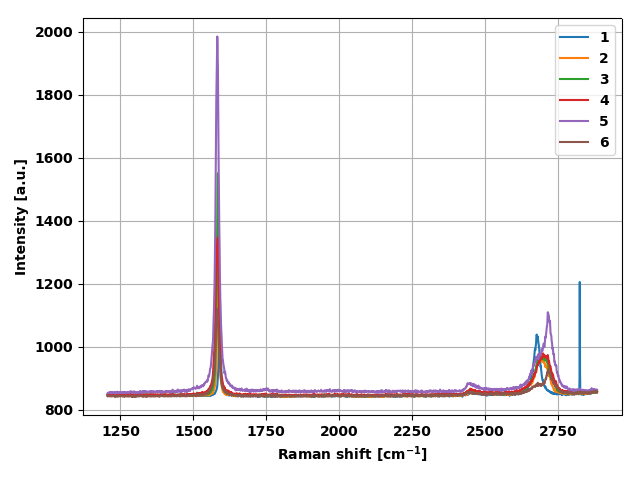
\includegraphics[scale=0.5]{Bilder/Exfoliation/2_mono_bi_tri_flake_all.PNG}
\caption{Raman spectra from the flake shown in Fig. \ref{fig:Exfoliation_Microscope}.}
\label{fig:Exfoliation_Spectra}
\end{figure}

Figure \ref{fig:Exfoliation_Spectra} shows the Raman spectra at the measurement points as shown in figure \ref{fig:Exfoliation_Microscope}. \\
As one can hardly see the intensity of the G peak increases with increasing number of layer until its saturation. But the shape and position are for all measurement points approximately identical. The 2D peaks though are approximately at the same position, but the intensity and the shape vary. The shape variation is a hint to different strain, as the 2D peak with strain gets a superposition of two postponed peaks. 



\section{Half Sandwich on PMMA}
A graphene flake is placed on a hexagonal boron nitride (hBN) film, which is applied on a Polymethylmethacrylat (PMMA) sample. 

\subsection{Single Spectra}

\begin{figure}
\centering
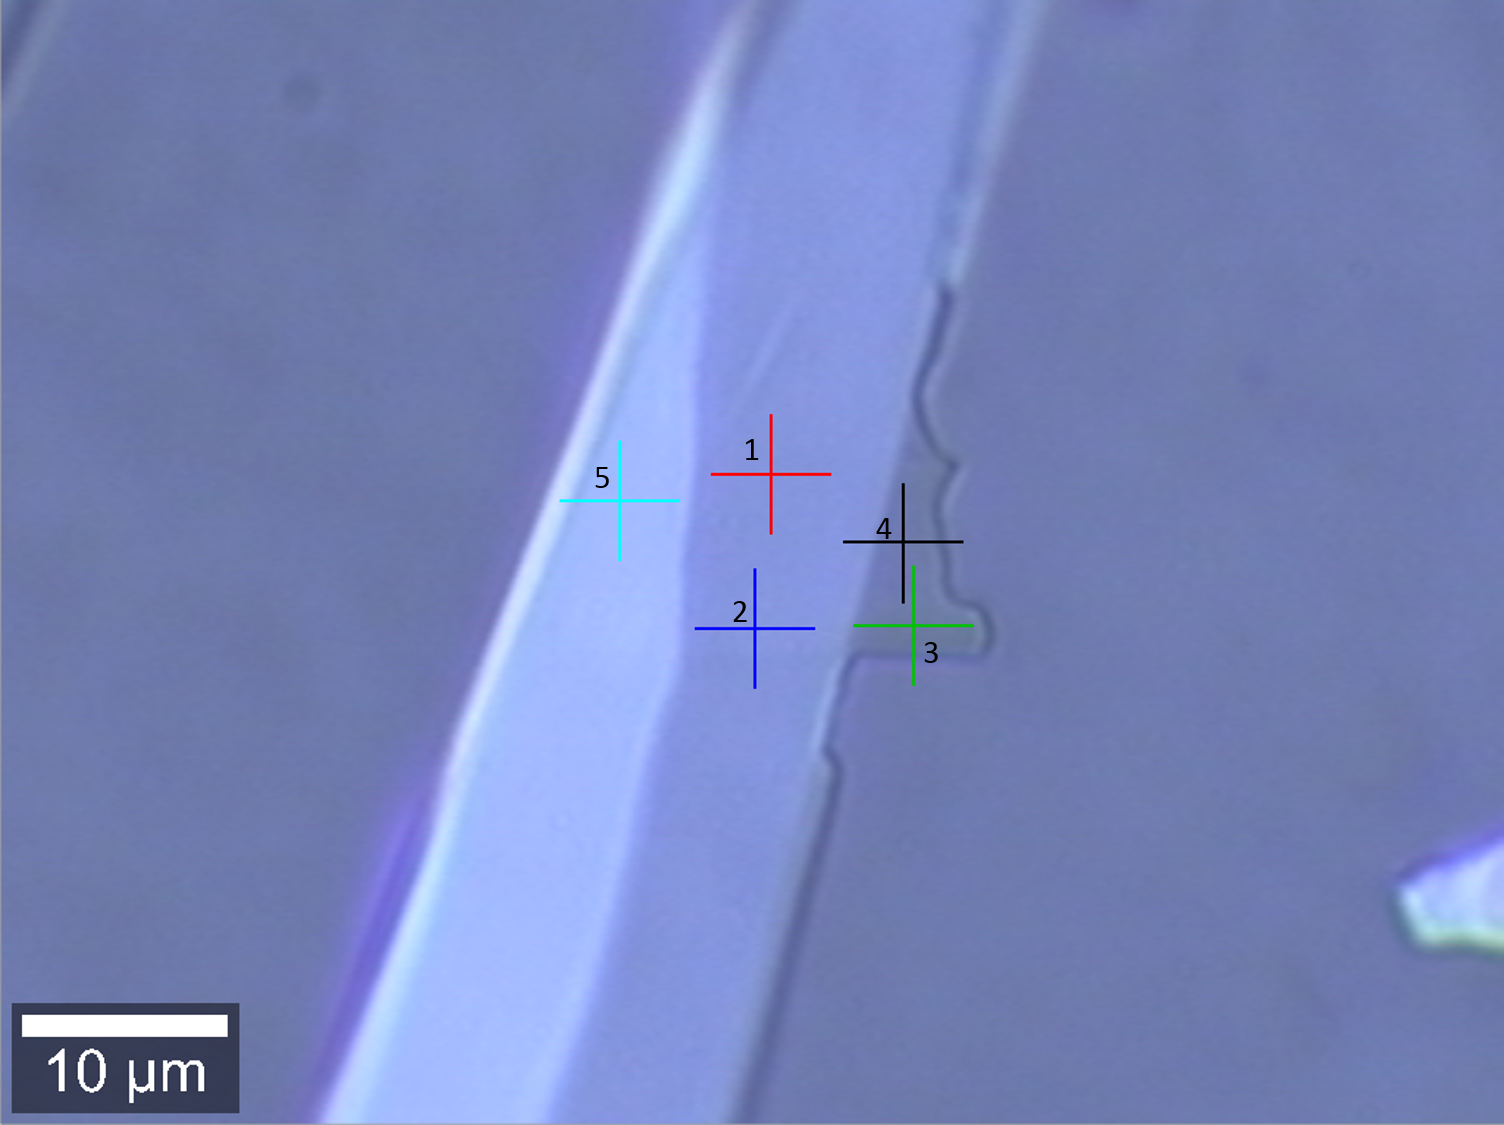
\includegraphics[scale=0.25]{Bilder/Part_2/4_Half_sandwich_on_PMMA.PNG}
\caption{Image from one graphene hBn sandwich made with an optical microscope. The crosses mark the points where the Raman spectra are extracted.}
\label{fig:Part2_map_microscope}
\end{figure}

\begin{table}[h]
\centering
\begin{tabular}{|c|c|c|c|c|}
\hline 
Measurement & $\omega _G$ & $\Gamma _G$ & $\omega _{2D}$ & $\Gamma _{2D}$ \\ 
point &  &  &  &  \\ 
\hline 
1 & \SI{1584.25 \pm 0.15}{\per cm} & \SI{12.57 \pm 0.25}{\per cm} & \SI{2680.89 \pm 0.16}{\per cm} & \SI{17.19 \pm 0.52}{\per cm} \\ 
\hline 
2 & \SI{1582.95 \pm 0.16}{\per cm} & \SI{11.59 \pm 0.13}{\per cm} & \SI{2695.50 \pm 0.35}{\per cm} & \SI{50.37 \pm 0.49}{\per cm} \\ 
\hline 
3 & \SI{1582.44 \pm 0.17}{\per cm} & \SI{13.68 \pm 0.11}{\per cm} & \SI{2694.61 \pm 0.27}{\per cm} & \SI{52.02 \pm 0.36}{\per cm} \\ 
\hline 
4 & \SI{1583.30 \pm 0.55}{\per cm} & \SI{16.26 \pm 0.10}{\per cm} & \SI{2693.79 \pm 0.29}{\per cm} & \SI{35.06 \pm 0.43}{\per cm} \\ 
\hline 
5 & \SI{1583.32 \pm 0.21}{\per cm} & \SI{12.31 \pm 0.25}{\per cm} & \SI{2692.23 \pm 0.16}{\per cm} & \SI{13.09 \pm 0.23}{\per cm} \\ 
\hline 
\end{tabular} 
\caption{Results for the positions and width of G and 2D peak from the spectra at the measurement points as marked in Fig. \ref{fig:Part2_map_microscope}.}
\label{tab:Sandwich_Results}
\end{table}

Table \ref{tab:Sandwich_Results} shows the measured positions and width of the G and 2D peak at every measurement point as marked in figure \ref{fig:Part2_map_microscope}. \\
As one can see the position of the G peak differs only a little bit. The width of the G peak sway around approximately 20\%. \\
The magnitude of the variation of the 2D peak position is similar to the one from the G peak. The width of the G peak is variing a lot more than the one of the 2D peak.


\subsection{$\Gamma _{2D}$ map}

\begin{figure}
\centering
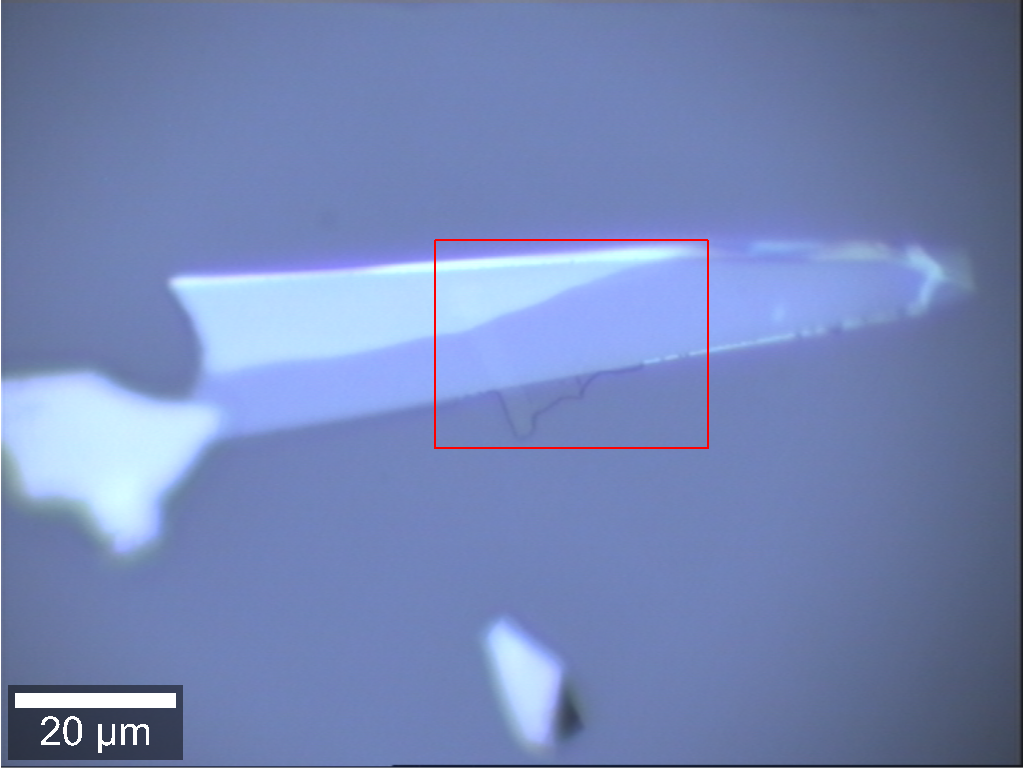
\includegraphics[scale=0.2]{Bilder/Part_2/half_sandwich_map.PNG}
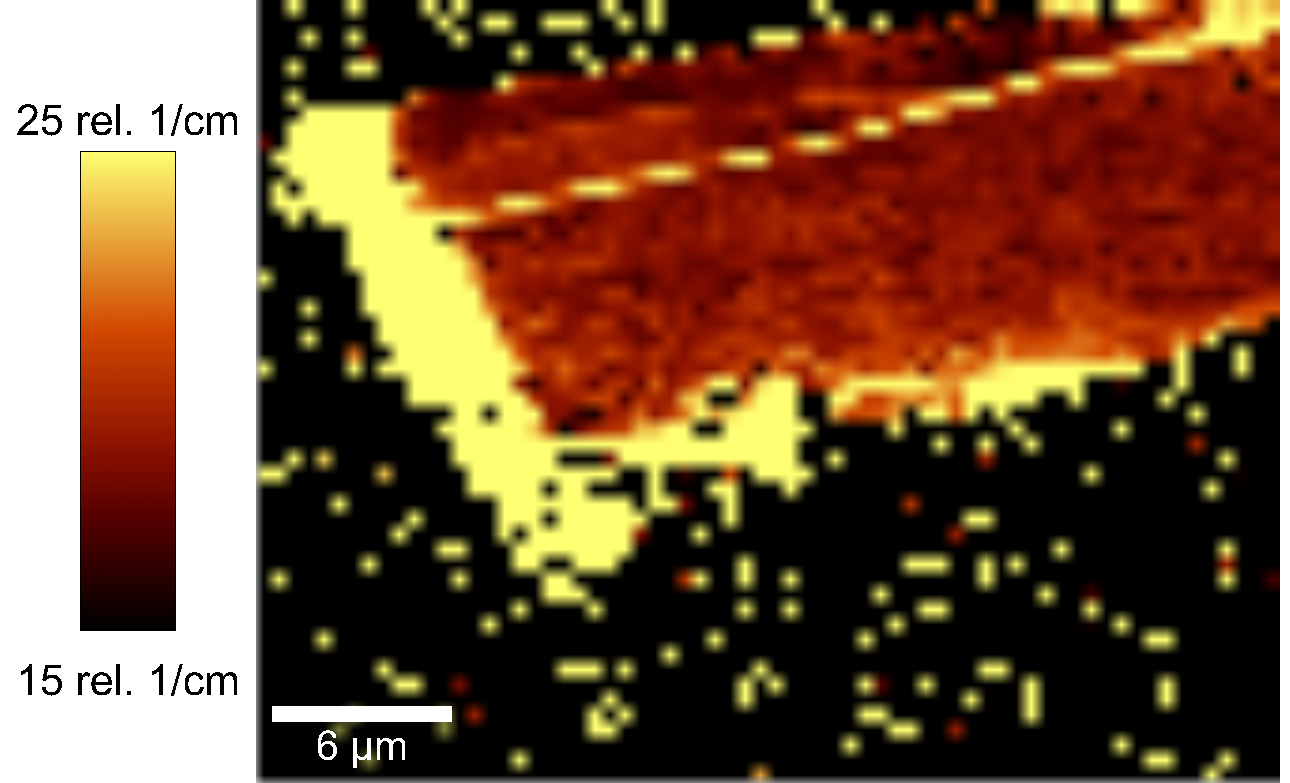
\includegraphics[scale=0.2]{Bilder/Part_2/half_sandwich_map_2D_width.PNG}
\caption{The upper image shows the microscope image of the flake. The lower image shows the map of $\Gamma _{2D}$ from the red boxed part.}
\label{fig:Part2_map}
\end{figure}

Figure \ref{fig:Part2_map} shows a $\Gamma _{2D}$ map of the same flake as analyzed with the five single spectra before. \\
On the map one can see a superposition of the structure of the graphene flake and the structure of the hBn. Those areas on which graphene and hBn are present are colored red which corresponds to a $\Gamma _{2D}$ of around \SI{20}{\per cm}. Where neither of those are present the color is black which corresponds to a $\Gamma _{2D}$ of around \SI{15}{\per cm}. The edges of the graphene flake are colored yellow which corresponds to a $\Gamma _{2D}$ of around \SI{25}{\per cm}.




















\bibliography{Raman}% Produces the bibliography via BibTeX.

\end{document}
